% %!TEX root = ../thesis.tex
% % ******************************* Thesis Appendix B ********************************

\chapter{IARIA}
\label{AppendixB}
\textbf{Journal paper published in The International Journal of Advances in Security} \\

The Internation Journal of Advances in Security publishes special issues, from time to time, that draws contributions from its sister conferences. Such contributions are selected by the editors of the journal based on the publications in the proceedings of the conferences. Based on the the relevance and recommendations from the peer review process, selected papers are invited to be extended for inclusion in the special issues of the journal.

The conference paper in Appendix A was selected for publication in the International Journal of Advances in Security and is subsequently presented here in Appendix B. The main results of the study were presented in this paper. Before publication, the paper subjected to a double-blind peer review.\\

\textit{Contributions of authors:}
\begin{itemize}
    \item[--] Shahim, Louis-Philip - Principle investigator and lead author
    \item[--] Snyman, Dirk - Supervisor and experimental design
    \item[--] Du Toit, Tiny - Co-supervisor and critical reader (technical)
    \item[--] Kruger, Hennie - Co-supervisor and critical reader (conceptual)
\end{itemize}

\textbf{Bibliographic reference:} Shahim, L.P.; Snyman, D.P.; Du Toit, J.V.; Kruger, H.A. Cancelable hand geometry-based biometric authentication system using steganography techniques. \textit{International Journal of Advances in Security}, 2017, 10, pp. 134-144.

% Paper published in the International Journal of Advances in Security 10 (3 \& 4), 134-144. This journal article was written under invitation to do so and was subject to peer review.

% This paper involved the bulk of the literature review and has been the greatest contribution to this particular study. The development of the proposed framework was primarily based on the findings mentioned here.

% This journal article was presented at the 44th ORSA conference in 2017. Valuable insights were gained from that conference and the necessary applications and adjustments were made to the study for the better.

% The final journal article can be seen on the pages that follow.

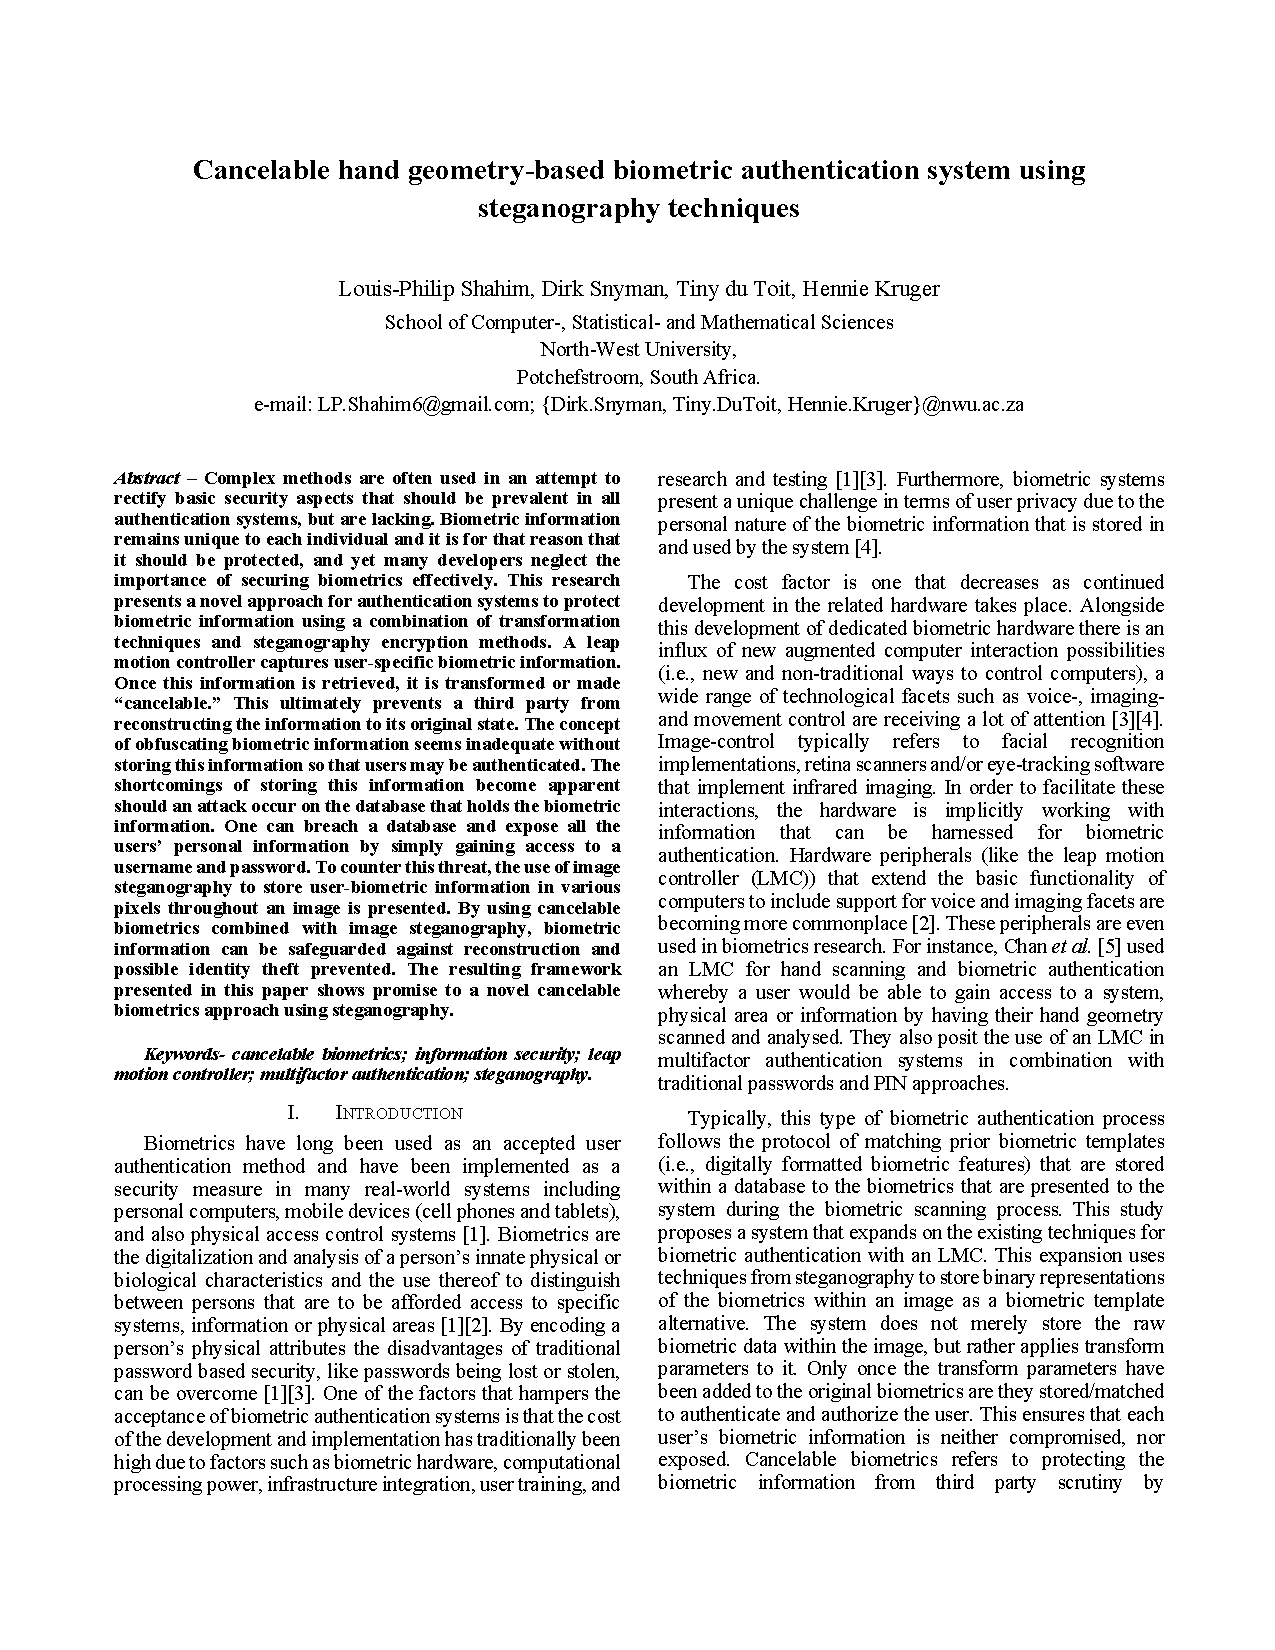
\includepdf[pages=1-,pagecommand={}]{Appendix2/IARIA.pdf}
% 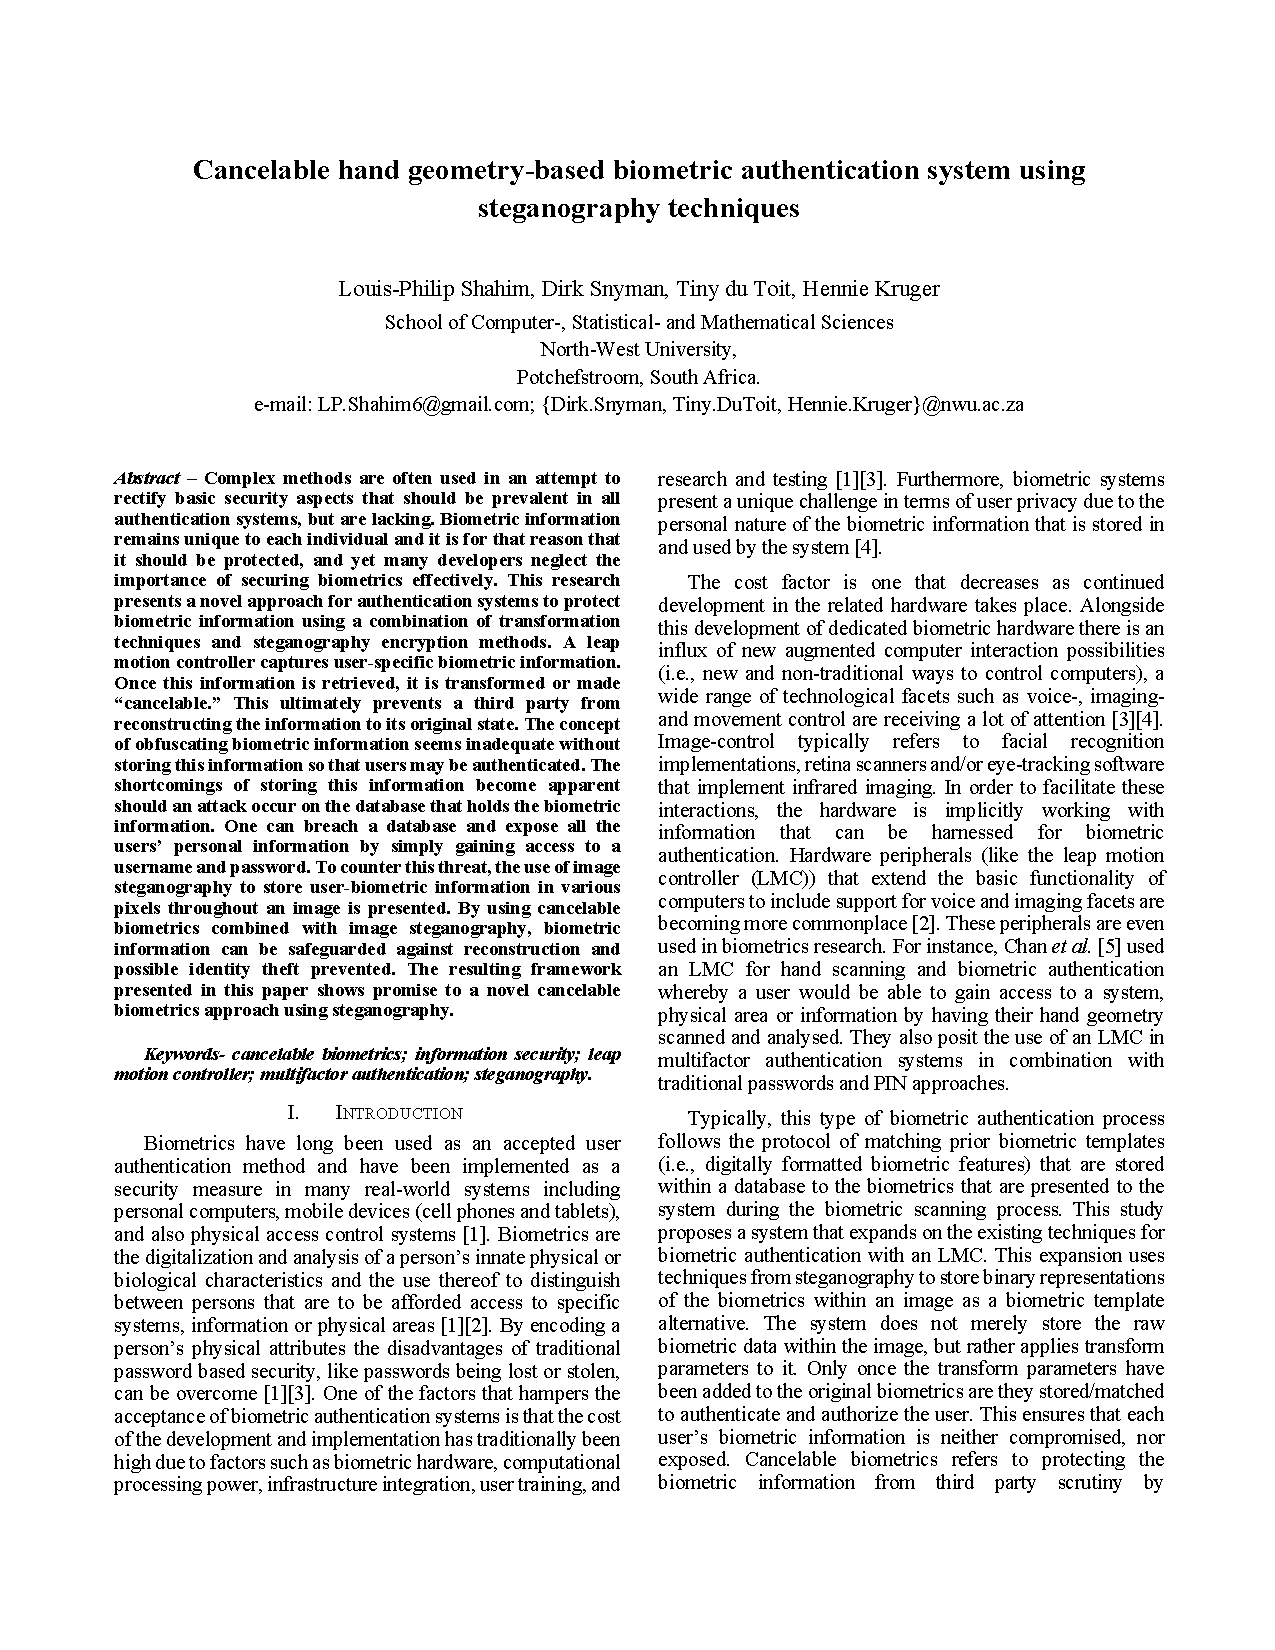
\includepdf[pages=1,scale=.8,pagecommand={\section{Appendix B:} }]{Appendix2/IARIA.pdf}
% \includepdf[pages=2-,pagecommand={}]{Appendix2/IARIA.pdf}
